\subsection{Lapsus}
Something about what we used from state of art
\subsubsection{Board and sensors}
Something about the board we use and what sensors it have and why we chose that. We use the ESP32-C6-DEV bord and the accration sensor.
\subsubsection{I2C og SPI}
\subsubsection{Fall detection algorithm}
Something about why are we using threshold detection
\begin{itemize}
    \item Long battery life  
    \item Simple and reliable  
    \item Low board power consumption
\end{itemize}

\subsubsection{The fall}
The paper \cite{hsieh_novel_2017} describe a fall as a sequence of three distinct phases seen in the figure: \ref{fig:sensor_fall_graph}.

\begin{figure}
    \centering
    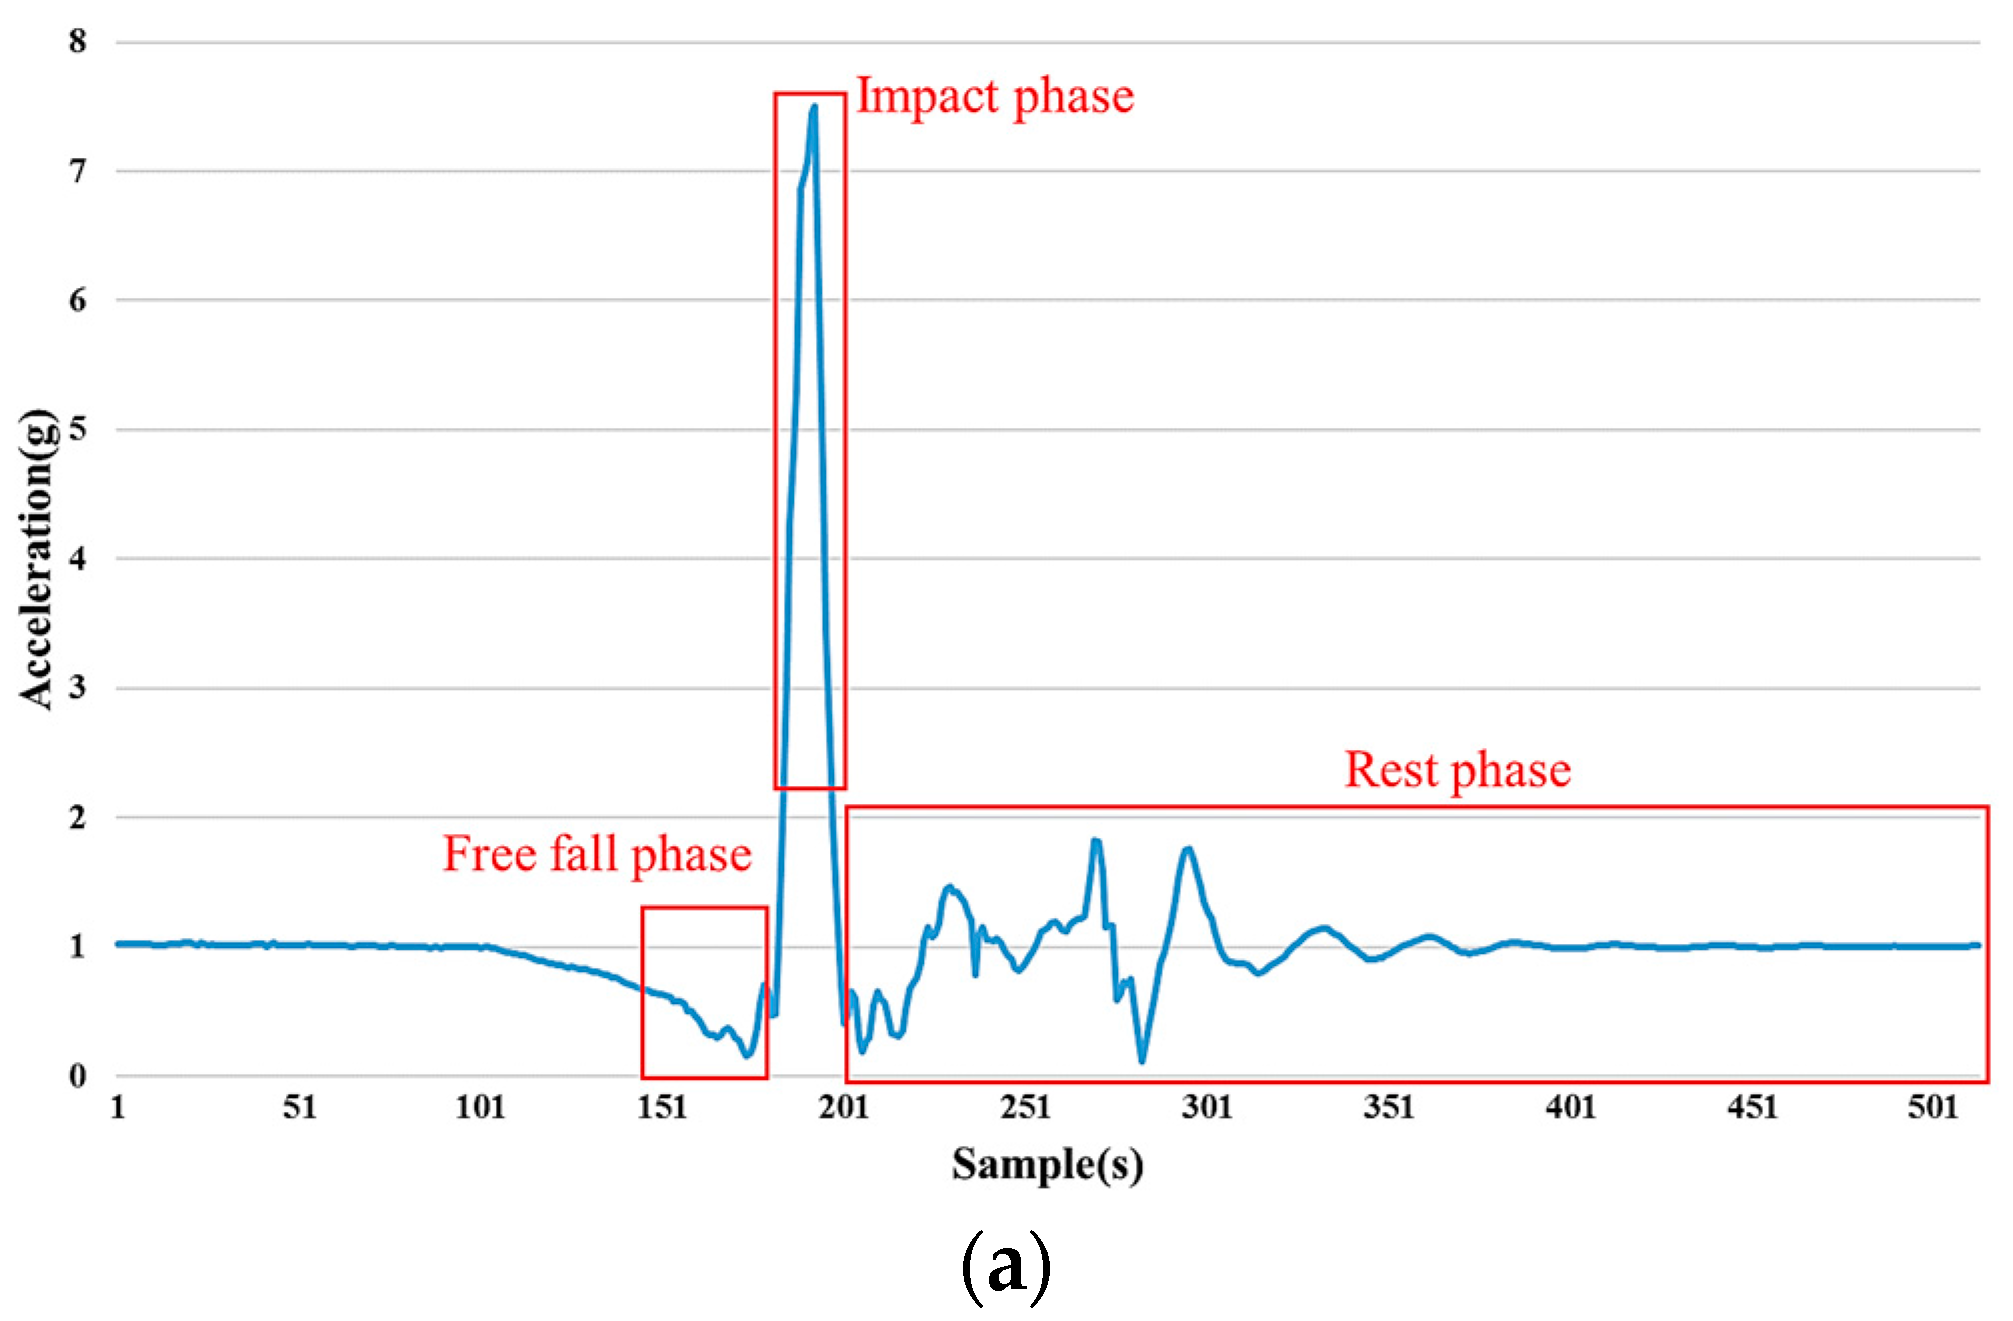
\includegraphics[width=0.75\linewidth]{report/images/sensor_fall_graph.png}
    \caption{Illustration showing a standing forward fall and the tree phases of a fall from \cite{hsieh_novel_2017}.}
    \label{fig:sensor_fall_graph}
\end{figure}

\paragraph{Free fall}
During free fall, the accelerometer experiences a rapid drop in measured acceleration, often approaching 0 g. This occurs because the body is no longer supported by the ground, causing the sensor to be in a near-weightless state. Detecting this drop is a strong early indicator that a fall may be occurring.

\paragraph{Impact}
The impact phase is characterized by a sudden and sharp spike in acceleration as the body collides with the ground or another surface. This spike typically exceeds a predefined threshold, making it the most distinct and reliable indicator of a fall event.

\paragraph{Rest}
After the impact, the body enters a rest phase where movement decreases significantly. The accelerometer readings stabilize, often showing minimal variation. Monitoring this phase helps distinguish real falls from false positives, as genuine falls usually include a period of low movement following the impact.

\subsubsection{Emergency button}
Something about how the button work 

\subsubsection{Hard impact}
Something about how it detects hard impacts

\subsection{Bluetooth}
How the Bluetooth are setup using NimBLE.

\subsubsection{User service}
Something about the fall characteristic, impact characteristic and emergency button characteristic.

\subsubsection{Battery service}
Something about the battery characteristic and how battery are calculated.